
%% bare_jrnl.tex
%% V1.3
%% 2007/01/11
%% by Michael Shell
%% see http://www.michaelshell.org/
%% for current contact information.
%%
%% This is a skeleton file demonstrating the use of IEEEtran.cls
%% (requires IEEEtran.cls version 1.7 or later) with an IEEE journal paper.
%%
%% Support sites:
%% http://www.michaelshell.org/tex/ieeetran/
%% http://www.ctan.org/tex-archive/macros/latex/contrib/IEEEtran/
%% and
%% http://www.ieee.org/



% *** Authors should verify (and, if needed, correct) their LaTeX system  ***
% *** with the testflow diagnostic prior to trusting their LaTeX platform ***
% *** with production work. IEEE's font choices can trigger bugs that do  ***
% *** not appear when using other class files.                            ***
% The testflow support page is at:
% http://www.michaelshell.org/tex/testflow/


%%*************************************************************************
%% Legal Notice:
%% This code is offered as-is without any warranty either expressed or
%% implied; without even the implied warranty of MERCHANTABILITY or
%% FITNESS FOR A PARTICULAR PURPOSE! 
%% User assumes all risk.
%% In no event shall IEEE or any contributor to this code be liable for
%% any damages or losses, including, but not limited to, incidental,
%% consequential, or any other damages, resulting from the use or misuse
%% of any information contained here.
%%
%% All comments are the opinions of their respective authors and are not
%% necessarily endorsed by the IEEE.
%%
%% This work is distributed under the LaTeX Project Public License (LPPL)
%% ( http://www.latex-project.org/ ) version 1.3, and may be freely used,
%% distributed and modified. A copy of the LPPL, version 1.3, is included
%% in the base LaTeX documentation of all distributions of LaTeX released
%% 2003/12/01 or later.
%% Retain all contribution notices and credits.
%% ** Modified files should be clearly indicated as such, including  **
%% ** renaming them and changing author support contact information. **
%%
%% File list of work: IEEEtran.cls, IEEEtran_HOWTO.pdf, bare_adv.tex,
%%                    bare_conf.tex, bare_jrnl.tex, bare_jrnl_compsoc.tex
%%*************************************************************************

% Note that the a4paper option is mainly intended so that authors in
% countries using A4 can easily print to A4 and see how their papers will
% look in print - the typesetting of the document will not typically be
% affected with changes in paper size (but the bottom and side margins will).
% Use the testflow package mentioned above to verify correct handling of
% both paper sizes by the user's LaTeX system.
%
% Also note that the "draftcls" or "draftclsnofoot", not "draft", option
% should be used if it is desired that the figures are to be displayed in
% draft mode.
%
\documentclass[journal]{IEEEtran}
\usepackage{blindtext}
\usepackage{graphicx}
\usepackage{amsmath}
\usepackage{algpseudocode}% http://ctan.org/pkg/algorithmicx
\algtext*{EndWhile}% Remove "end while" text
\algtext*{EndIf}% Remove "end if" text


\begin{document}
%
% paper title
% can use linebreaks \\ within to get better formatting as desired
\title{Restricted Boltzmann Machines}


\author{Jason~Liang,
        Julian~Sia% <-this % stops a space
% \thanks{M. Shell is with the Department
% of Electrical and Computer Engineering, Georgia Institute of Technology, Atlanta,
% GA, 30332 USA e-mail: (see http://www.michaelshell.org/contact.html).}% <-this % stops a space
% \thanks{J. Doe and J. Doe are with Anonymous University.}% <-this % stops a space
% \thanks{Manuscript received April 19, 2005; revised January 11, 2007.}
}

% note the % following the last \IEEEmembership and also \thanks - 
% these prevent an unwanted space from occurring between the last author name
% and the end of the author line. i.e., if you had this:
% 
% \author{....lastname \thanks{...} \thanks{...} }
%                     ^------------^------------^----Do not want these spaces!
%
% a space would be appended to the last name and could cause every name on that
% line to be shifted left slightly. This is one of those "LaTeX things". For
% instance, "\textbf{A} \textbf{B}" will typeset as "A B" not "AB". To get
% "AB" then you have to do: "\textbf{A}\textbf{B}"
% \thanks is no different in this regard, so shield the last } of each \thanks
% that ends a line with a % and do not let a space in before the next \thanks.
% Spaces after \IEEEmembership other than the last one are OK (and needed) as
% you are supposed to have spaces between the names. For what it is worth,
% this is a minor point as most people would not even notice if the said evil
% space somehow managed to creep in.

% make the title area
\maketitle

\begin{abstract}
In this report 
\end{abstract}

\IEEEpeerreviewmaketitle

\section{Introduction}
Restricted Boltzmann Machines (RBM) are a type of undirected graphical model consisting of two sets of nodes, a set of hidden units and a set of visible units.  Given the graph $G = (V,E)$ that describes the Restricted Boltzmann Machine, $\forall \, v_{vis} \: \epsilon \: V_{vis} \subset V,\exists e'\epsilon E$, such that $ e'=(v_{vis}, v_{hid}),\: \forall \, v_{hid} \, \epsilon \, V_{hid} \subset V$.  Restricted Boltzmann Machines are a variant of the Boltzmann Machine posed by Hinton and Sejnowski \cite{ackley1985learning}, with the restriction that there are neither edges connecting any visible units nor edges connecting any hidden units.  This restriction guarantees that the visible units are conditionally independent of other visible units; and hidden units, conditionally independent of hidden units. Restricted Boltzmann Machines today are commonly used in classification tasks, dimensionality reduction, and feature learning tasks.

\section{Previous Work}
Restricted Boltzmann Machines were created as a variant of Boltzmann Machines after practical difficulties were encountered in training Boltzmann machines, namely the exponential training time required to learn weights in a Boltzmann Machine and sequential nature of training particular to the Boltzmann Machine.  Boltzmann Machine themselves were motivated primarily by limitations of Hopfield Networks \cite{hopfield1985neural}, primarily their poor storage capacity and tendency to converge at local energy minima.  

In the early days of Boltzmann machines, Hinton and Sejnowski calculated the gradient of the log likelihood by ``[fixing] a training vector on the visible units, initializing the hidden units to random binary states, and using sequential Gibbs sampling of the hidden units" \cite{ackley1985learning}, using simulated annealing to speed up the convergence process.  Other attempts were made by Neal with persistent Markov chains \cite{neal1992connectionist} and Peterson and Anderson with mean-field methods (instead of Gibbs Sampling) to speed up the learning process \cite{peterson1987mean}. After Restricted Boltzmann Machines were posed as a simplifying restriction by Smolensky, Hinton discovered a way to speed up the learning process, coined ``contrastive divergence," which is described in this report \cite{hinton2006fast,hinton2010practical}.

\section{Algorithm Description}
Given a set of training vectors, V, to train a Restricted Boltzmann, one aims to maximize the average log probability, $p(v), v \epsilon V$, where
\begin{equation}
p(v) = \frac{1}{Z} \sum\limits_{h} e^{-E(v,h)},\;
Z = \sum\limits_{v,h} e^{-E(v,h)}
\end{equation}
One can do accomplish this by taking the derivative of the log probability of $p(v)$ with respect to the weights defined in the energy function, $E(v,h)$ defined as

\begin{equation}
\begin{aligned}
E(v,h) &= \:- \sum\limits_{i \, \epsilon \, visible} a_{i}v_{k} \: - \sum\limits_{j \, \epsilon \, hidden} b_{j}h_{j} \: - \sum\limits_{i}\sum\limits_{j} v_{i}w_{i,j}h_{j}\\
&=\: -b'v - c'h - h'Wv
\end{aligned}
\end{equation}

Differentiating with respect to $w_{i,j}$, we find that the partial derivative reduces to the following:

\begin{equation}
\begin{aligned}
\frac{\partial p(v)}{\partial w_{i,j}} & = {\langle v_{i} h_{j} \rangle}_{data} - {\langle v_{i} h_{j} \rangle}_{model} \\
\end{aligned}
\end{equation}

With this reduction the following learning rule with $\epsilon$ learning rate can be derived

\begin{equation}
\Delta w_{i,j} = \epsilon\langle{\langle v_{i} h_{j} \rangle}_{data} - {\langle v_{i} h_{j} \rangle}_{model}\rangle 
\end{equation} 

Alternatively, using free energy notation, the partial derivative can be defined as
\begin{equation}
\begin{aligned}
- \frac{\partial p(v)}{\partial \Theta} = \frac{\partial \mathcal{F}(v)}{\partial \Theta} - \sum\limits_{\tilde{v}}p(\tilde{v}) \frac{\partial \mathcal{F}(\tilde{v})}{\partial \Theta}
\end{aligned}
\end{equation} where we define free energy as 

\begin{equation}
\mathcal{F}(v) = -log \sum\limits_{h}e^{-E(v,h)}
\end{equation}

Because the computation of the second term in the difference that defines the partial derivative is intractable, we can approximate the second term using a fixed number of samples from the model, such that 

\begin{equation}
\begin{aligned}
- \frac{\partial p(v)}{\partial \Theta} = \frac{\partial \mathcal{F}(v)}{\partial \Theta} -\frac{1}{|\mathcal{N}|} \sum\limits_{\tilde{v} \epsilon \mathcal{N}} p(\tilde{v}) \frac{\partial \mathcal{F}(\tilde{v})}{\partial \Theta}
\end{aligned}
\end{equation}

In the case of a binary Restricted Boltzmann Machine, the free energy function reduces to the following:

\begin{equation}
\begin{aligned}
\mathcal{F}(v) = -b'v - \sum\limits_{i}log\sum\limits_{h_{i}}e^{h_{i}(c_{i}+W_{i}v)}
\end{aligned}
\end{equation}

Using the free energy function defined in (8) and the derivative defined in (7), we can define the following update equations for the Restricted Boltzmann Machine's log likelihood gradient:

\begin{equation}
\begin{aligned}
- \frac{\partial p(v)}{\partial W_{i,j}} &= E_{v}[p(h_{i}|v)\cdot v_{j}] - v_{j}^{(i)}\cdot sigm(W_{i} \cdot v^{(i)} + c_{i})\\
- \frac{\partial p(v)}{\partial c_{i}} &= E_{v}[p(h_{i}|v)] - v_{j}^{(i)}\cdot sigm(W_{i} \cdot v^{(i)})\\
- \frac{\partial p(v)}{\partial b_{j}} &= E_{v}[p(h_{i}|v)] - v_{j}^{(i)}
\end{aligned}
\end{equation}

To obtain samples from p(x), one can use Gibbs sampling until a Markov chain converges or near converges.  Because of the conditional independence assumptions of the visible and hidden nodes such that 

\begin{equation}
\begin{aligned}
p(h|v) = \prod\limits_{i} p(h_{i}|v)\\
p(v|h) = \prod\limits_{j} p(v_{j}|h)
\end{aligned}
\end{equation} we can define the following activation functions:

\begin{equation}
\begin{aligned}
p(h_{i} = 1|v) = sigm(c_{i} + W_{i}v)\\
p(v_{j} = 1|j) = sigm(b_{j} + W_{i}'h)
\end{aligned}
\end{equation}

Given the conditional independence assumptions of the Restricted Boltzmann Machine, we can perform block Gibbs Sampling with the following update rules:

\begin{equation}
\begin{aligned}
h^{(n+1)} \sim sigm(W'v^{(n)} + c)\\
v^{(n+1)} \sim sigm(Wh^{(n+1)} + b)
\end{aligned}
\end{equation}

As $t \rightarrow \infty,  (v^{(t)},h^{(t)})$, the samples of $p(v,h)$ will be accurate.  Nevertheless, one can further speed up the process by using the "contrastive divergence," which involves initializing the Markov chain with a training example $v \epsilon V$ and running the Markov chain for k (often with $k = 1$) iterations.  In the context of the derivative defined in (7), contrastive divergence can be roughyl outlined as the following:

\begin{enumerate}
 \item Replace the first term (expectation over all input samples) with a single sample.
 \item For the second term, run the Markov chain for fixed $k$ steps.
\end{enumerate}

More explicitly, contrastive divergence can be described as the following:

\begin{enumerate}
\item Take a training sample $v$, compute the probabilities of the hidden units and sample a hidden activation vector $h$ from this probability distribution.
\item Compute the outer product of $v$ and $h$ and call this the positive gradient.
\item From $h$, sample a reconstruction $v'$ of the visible units, then resample the hidden activations $h'$ from this. (Gibbs sampling step)
\item Compute the outer product of $v'$ and $h'$ and call this the negative gradient.
\item Let the weight update to $w_{i,j}$ be the positive gradient minus the negative gradient, times some learning rate (see equation (4)). 
\end{enumerate}

\section{Recent Applications}
One of the more recent applications of Restricted Boltzmann Machines is their use in stacks.  By stacking Restricted Boltzmann Machines, hidden layers can be trained on top of other hidden layers. After training multiple hidden layers, these layers can be unrolled to form a deterministic deep neural network.  A deep neural network of such variety can then be finely tuned with common training methods such as backpropagation.  In 2006, Hinton, using a similar structure alluded to here, trained a deep neural network, which achieved an error rate of 1.39\%, which outperformed a SVM with RBF kernel, which were considered state of the art at the time \cite{hinton2006fast}.

\begin{figure}[h]
  \centering
  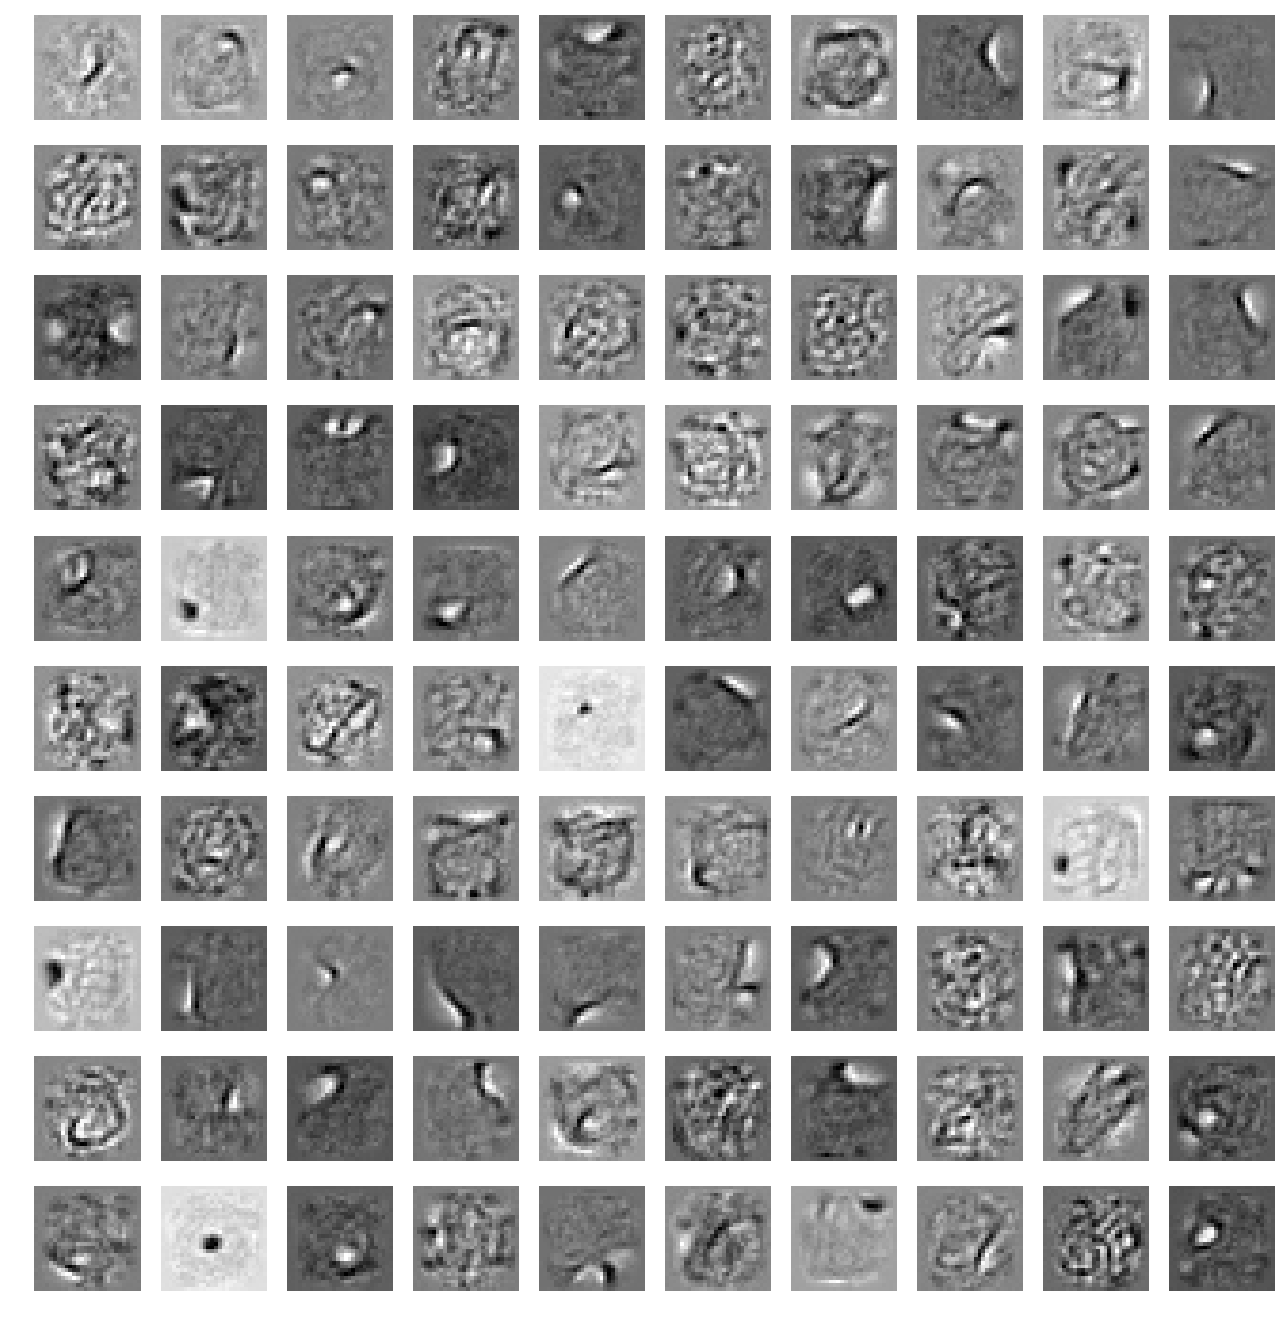
\includegraphics[width=0.9\linewidth]{filters.png}
  \caption{Filters corresponding the weights of the first 100 hidden nodes.}
  \label{filters}
\end{figure}

\section{Experimental Results}
We implement our own Restricted Boltzmann Machine in Python with the NumPy library \cite{oliphant2006guide}. We train a RBM with 784 visible units and 500 hidden units on the MNIST handwritten digit dataset \cite{deng2012mnist}, a standard benchmark for image classification. The learning algorithm used is CD-1, which is the simplest of the contrastive divergence methods but tends to work very well in practice. We initialize the weights of the RBM randomly by sampling them from a normal distribution with zero mean and 0.01 standard deviation. Next, we apply CD-1 to all 60,000 training images for 15 epochs with a learning rate 0.005.

In Fig.~\ref{filters}, we visualize the trained weights of the RBM. Each hidden node is connected to all 784 visible nodes and thus we can display the weights corresponding to a hidden node as an image with the same dimension as the input digits. As shown by the figure, the filters learned are interesting, with a diverse variety of different edge and blob detectors. 

Next in Fig.~\ref{samples}, we show the samples generated by the RBM when given test digits as input. The first column shows the original digits while the subsequent columns shows samples outputted by the model after an interval of 1000 steps of Gibbs sampling (to ensure proper mixing of the Markov chain). The images in Fig.~\ref{samples} show that RBM has properly learned the distribution for input digits and that samples are drawn from that distribution properly. 

\begin{figure}[h]
  \centering
  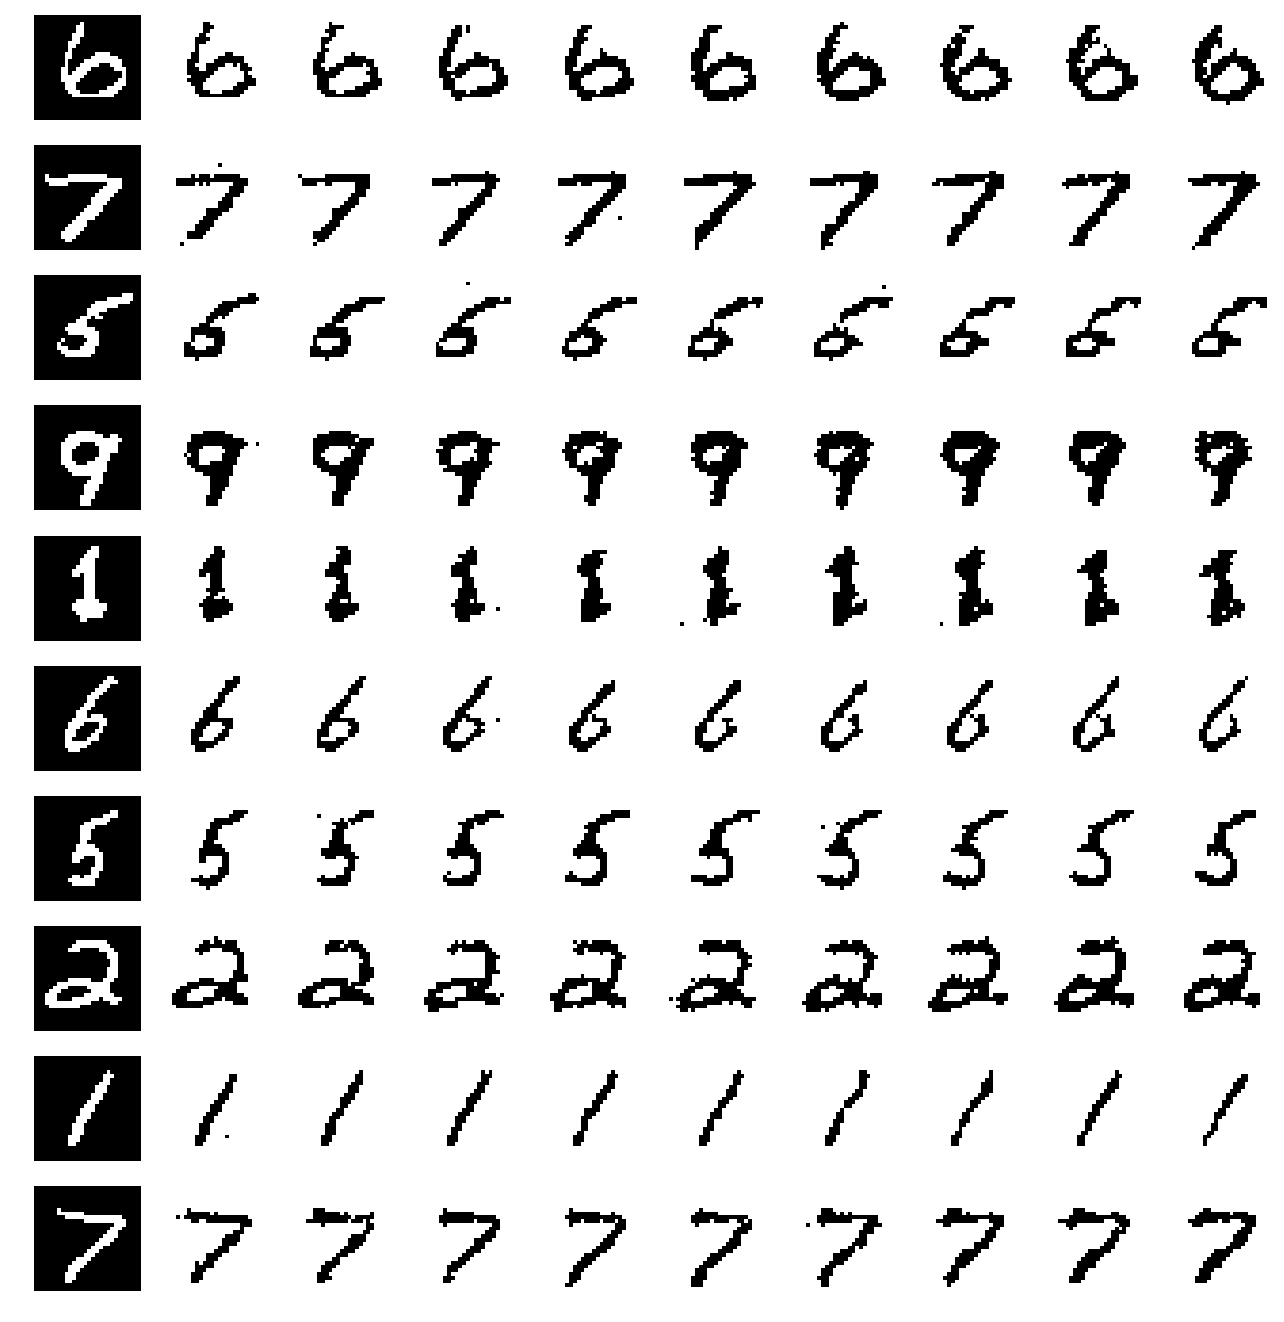
\includegraphics[width=0.9\linewidth]{samples.png}
  \caption{Samples generated by RBM. The first column shows original test digit sample. Subsequent columns show digits sampled from RBM with an interval of 1000 steps of Gibbs sampling.}
  \label{samples}
\end{figure}

Lastly, we explore the usefulness of RBMs in learning good representations of the input data and performing dimensionality reduction. As a preprocessing step prior to classification, we treat our trained RBM as a deterministic single layer neural network and use it to transform the input digits into a 500 dimensional feature vector. This feature vector is then used for supervised training of a logistic regression classifier. Without an RBM layer, the misclassification rate on a test set of 10,000 digits is 8.20\%. With the addition of the RBM layer, the error rate of the logistic regression classifier decreases to 3.07\%, an relative improvement of over 150\%.

\section{Conclusion}
As demonstrated in previous research and in our explorations, Restricted Boltzmann Machines are quite useful for classification tasks. With their relatively simple training procedures and given recent innovations in the use of Restricted Boltzmann Machines, Restricted Boltzmann machines have promising future uses in deep neural networks.



% trigger a \newpage just before the given reference
% number - used to balance the columns on the last page
% adjust value as needed - may need to be readjusted if
% the document is modified later
%\IEEEtriggeratref{8}
% The "triggered" command can be changed if desired:
%\IEEEtriggercmd{\enlargethispage{-5in}}

% references section

% can use a bibliography generated by BibTeX as a .bbl file
% BibTeX documentation can be easily obtained at:
% http://www.ctan.org/tex-archive/biblio/bibtex/contrib/doc/
% The IEEEtran BibTeX style support page is at:
% http://www.michaelshell.org/tex/ieeetran/bibtex/
%\bibliographystyle{IEEEtran}
% argument is your BibTeX string definitions and bibliography database(s)
%\bibliography{IEEEabrv,../bib/paper}
%
% <OR> manually copy in the resultant .bbl file
% set second argument of \begin to the number of references
% (used to reserve space for the reference number labels box)
\bibliographystyle{unsrt}
\bibliography{main}

% that's all folks
\end{document}
